\section{Verifying calibration}
\label{sec:verifying_calibration}

If a model outputs values from some finite set $S$,\footnote{The model can choose the set $S$.} and the probability of outputting each value $s \in S$ is not too small, then we can estimate its calibration error. The plugin estimator used in past work requires samples proportional to the number of model outputs $|S|$. Instead, we introduce the \emph{cancelling} estimator that requires samples proportional to $\sqrt{|S|}$. At a high level, the cancelling estimator leverages cancellation of error terms across different bins.

% We prove these finite sample guarantees (Theorem~\ref{thm:final-ours}), and show experimental evidence that our estimators approximate the calibration error better. We also show, experimentally, that using a better estimator allows us to pick out better models.

The plugin estimator directly estimates each term in the $\ell_2^2$ calibration error from samples~\cite{nguyen2015posterior, hendrycks2019anomaly, kuleshov2015calibrated, hendrycks2019pretraining}. Suppose we wish to measure the calibration error of a model $f : \mathcal{X} \to S$ where $S \subseteq [0, 1]$. Order the elements in $S$: $s_1 < s_2 < \dots < s_B$, where $B = |S|$ denotes the number of model outputs. Suppose we get an evaluation set $T_n = \{(x_1, y_1), \dots, (x_n, y_n)\}$ sampled i.i.d. from $P(X, Y)$.

\begin{definition}[Plugin estimator]
\label{dfn:plugin-estimator}
Let $L_i = \{ y_j \; | \; (x_j, y_j) \in T_n\wedge f(x_j) = s_i \}$ denote the label values where the model outputs $s_i$.

We estimate $E[Y | f(X) = s_i]$ as:
\[ \hat{y_i} = \sum_{y \in L_i} \frac{y}{|L_i|} \] 
We estimate $P(f(X) = s_i)$ by:
\[ \hat{p_i} = \frac{|L_i|}{n} \]
Then the plugin estimator for the $\ell_2^2$ error is:
\[ \hat{E}_{pl}^2 = \sum_{i=1}^b \hat{p_i} (s_i - \hat{y_i})^2 \]
\end{definition}

We now define our improved cancelling estimator. The key insight is that the plugin estimate of the error in each bin, $(s_i - \hat{y_i})^2$ is biased. By debiasing these estimates we get cancellations across bins.

\begin{definition}[Cancelling estimator]
The cancelling estimator for the $\ell_2^2$ error is:
\[ \hat{E}^2 = \sum_{i=1}^b \hat{p_i} \Big[ (s_i - \hat{y_i})^2 - \frac{\hat{y_i}(1 - \hat{y_i})}{\hat{p_i}n-1} \Big] \]
\end{definition}

The main results are that to check if the $\ell_2^2$ calibration error of a model is $\leq \epsilon^2$, the plugin estimator requires $\Theta(\frac{B}{\epsilon^2})$ samples (Theorem~\ref{thm:final-plugin}) while our estimator requires $\theta(\frac{\sqrt{B}}{\epsilon^2})$ samples (Theorem~\ref{thm:final-ours}). We begin by giving a bound on the error of the plugin estimator.

% An important condition for verifying calibration is $p_i$ cannot be too small.

% \begin{definition}
% \label{dfn:low-bal}
% We say a model is $k$-lower-balanced if $p(X = s_i) \geq \frac{1}{kB}$ for all $i$.
% \end{definition}
 
% We now analyze the two estimators. 

% \textbf{We use the following notation simplification} to simplify the theorem statements and proofs:
% \[ p_i = P(f(X) = s_i) \]
% \[ y_i^* = \mathbb{E}[Y \; | \; f(X) = s_i] \]
% \[ e_i = (s_i - y_i^*) \]

% Then, if we let ${E^*}^2$ denote the actual $\ell_2^2$ calibration error, we have:
% \[ {E^*}^2 = \sum_{i=1}^b p_i e_i^2 \]
% \subsection{Analysis of plugin estimator}
% \begin{lemma}
% \label{lemma:c_n_lemma}
% For some $k > 1$, suppose $p_i \geq \frac{1}{kb}$ for all $i$. Then if $n \geq 3kb \log{\frac{2b}{\delta}}$, we have $P(\forall i . \; |p_i - \hat{p_i}| \leq c(n) p_i) \geq 1 - \delta$ where
% \[ c(n) = \sqrt{\frac{3kb \log{\frac{2b}{\delta}}}{n}} \]
% \end{lemma}

% \begin{lemma}
% The plugin estimator satisfies the following decomposition:
% \[ \hat{E}^2 = \underbrace{\sum_{i=1}^b \hat{p_i}e_i^2}_{(1)}  - \underbrace{2\sum_{i=1}^b \hat{p_i}e_i(\hat{y_i} - y_i^*)}_{(2)} + \underbrace{\sum_{i=1}^b \hat{p_i}(\hat{y_i} - y_i^*)^2}_{(3)} \]
% \end{lemma}

\begin{theorem}
\label{thm:plugin-bound}
Let $p_i = P(f(X) = s_i)$ and suppose $p_i \geq \frac{1}{n}$ for all $i$. Let $c(n)$ be defined as:
\[ c(n) = \sqrt{\frac{1}{n \min p_i} \log{\frac{B}{\delta}}} \]
Then for the plugin estimator, with probability at least $1 - 3\delta$,
\[ | \hat{E_{pl}}^2 - {E^*}^2 | \leq c(n){E^*}^2 + \sqrt{\frac{2(1+c(n)){E^*}^2}{n} \log{\frac{2}{\delta}}} + \frac{B}{2n} \log{\frac{2B}{\delta}} \]
% For some $k > 1$, suppose $p_i \geq \frac{1}{kb}$ for all $i$. Then for the plugin estimator, if $n \geq 3kb \log{\frac{2b}{\delta}}$, with probability at least $1 - 3\delta$:
% \[ | \hat{E_{pl}}^2 - {E^*}^2 | \leq c(n){E^*}^2 + \sqrt{\frac{2(1+c(n)){E^*}^2}{n} \log{\frac{2}{\delta}}} + \frac{b}{2n} \log{\frac{2b}{\delta}} \]
% Where $c(n)$ is defined in Lemma~\ref{lemma:c_n_lemma}
\end{theorem}

% Theorem~\ref{thm:plugin-bound} gives a sample complexity bound for the estimation error. In many cases we are interested in checking if our model has calibration error $\leq \epsilon$. In other words, we are given $\epsilon$. If the calibration error is $> \epsilon$, then with probability at least $1 - \delta$ we should output that it is not calibrated. $1-\delta$ is the significance of the test. If the calibration error is $< r\epsilon$, then with probability at least $1 - \delta'$, we should output that the model is calibrated. $1 - \delta'$ is the power at effect size $r < 1$. Typically, we will choose $\delta = \delta'$.

% Theorem~\ref{thm:final-plugin} presents an easier way to think about this bound. Given constant $0 < r < 1$, suppose we want to estimate ${E^*}^2$ within a constant multiplicative factor. That is, we want $r {E^*}^2 \leq \hat{E_{pl}}^2 \leq (1+r) {E^*}^2$.

% Another way to think about this is we are given $\epsilon$, and if the model's calibration error is $> (1+r)\epsilon$ we should say the model is not calibrated. If the calibration error is $< r\epsilon$

Typically, we are interested in checking if our model has calibration error $\leq \epsilon$. In other words, we are given $\epsilon, \delta > 0$ and effect size $0 < r < 1$. If the calibration error is $> \epsilon$, then with probability at least $1 - \delta$ we should output that it is not calibrated. If the calibration error is $< r\epsilon$, then with probability at least $1 - \delta$, we should output that the model is calibrated.

\begin{theorem}[Plugin bound]
\label{thm:final-plugin}
Suppose $\forall i.\;p_i \geq \frac{1}{2B}$ and $n = \Theta(\frac{B}{\epsilon^2})$ ignoring $\log$ factors. Then the plugin estimator can check if ${E^*}^2 \leq \epsilon^2$ with failure probability $\delta$, and constant effect size $r$. 
\end{theorem}

Another way of thinking about this is that if $n = \Theta(\frac{B}{{E^*}^2})$ then $r {E^*}^2 \leq \hat{E_{pl}}^2 \leq (1+r){E^*}^2$. Next we bound the error of the cancelling estimator.

% \begin{corollary}
% \label{cor:final-plugin}
% Using the plugin estimator $\hat{E}_{pl}$, if $n = \Theta(kb + \frac{b}{\epsilon^2})$ ignoring $\log$ factors, we can check if $|{E^*} | \leq \epsilon$ with significance and power $\delta$, and constant effect size $r$. 
% \end{corollary}

% \subsection{Analysis of our estimator}

\begin{theorem}
\label{thm:our-bound}
Let $p_i = P(f(X) = s_i)$ and suppose $p_i \geq \frac{1}{n}$ for all $i$. Let $c(n)$ be as defined in Theorem~\ref{thm:plugin-bound}.
Then for the cancelling estimator, with probability at least $1 - 4\delta$,
\[ | \hat{E}^2 - {E^*}^2 | \leq c(n){E^*}^2 + \sqrt{\frac{2(1+c(n)){E^*}^2}{n} \log{\frac{2}{\delta}}} + \frac{\sqrt{B}}{n}\log{\frac{4n}{\delta}} \log{\frac{2}{\delta}} + \frac{1}{n}\]
\end{theorem}

\begin{theorem}[Cancelling bound]
\label{thm:final-ours}
Suppose $\forall i.\;p_i \geq \frac{1}{2B}$ and $n = \Theta(B+\frac{\sqrt{B}}{\epsilon^2})$ ignoring $\log$ factors. Then the cancelling estimator can check if ${E^*}^2 \leq \epsilon^2$ with failure probability $\delta$ and constant effect size $r$. 
\end{theorem}

\subsection{Experiments}

We ran experiments on CIFAR-10 and Imagenet to compare the practical performance of the cancelling estimator and the plugin estimator. We split the validation set into two chunks $C_1$ and $C_2$. We use $C_1$ to re-calibrate and discretize a trained model using $B = 100$ bins. For varying values of $n$, we sample $n$ points, with replacement, from $C_2$, and estimate the calibration error using the cancelling estimator and the plugin estimator. We then compute the squared deviation of these estimates from the calibration error measured on the entire chunk $C_2$. We repeat this 1,000 times to get the mean squared deviation and confidence intervals. The results are in Figure~\ref{fig:mse_estimators}. In the Appendix, we include results for ImageNet, ablations on $B$, and we visualize the histogram of the deviations.

We also run a multi-class calibration experiment on CIFAR-10 to show that our estimator allows us to select models with a better Brier score subject to a given calibration constraint. As before, we split the validation set into $C_1$ and $C_2$. On $C_2$, we estimate the calibration error using the plugin and cancelling estimators and use 100 Bootstrap resamples to compute a 90\% upper confidence bound on the estimate. We compute the Brier scores and the upper bounds on the calibration error for $B = 10, 15, \cdots, 100$ and show the Pareto curve in Figure~\ref{fig:mse_vs_ce_estimators}. The results show that for any desired calibration error, the cancelling estimator enables us to pick out models with a better Brier score.

\begin{figure}
  \centering
  \centering
     \begin{subfigure}[b]{0.45\textwidth}
         \centering
         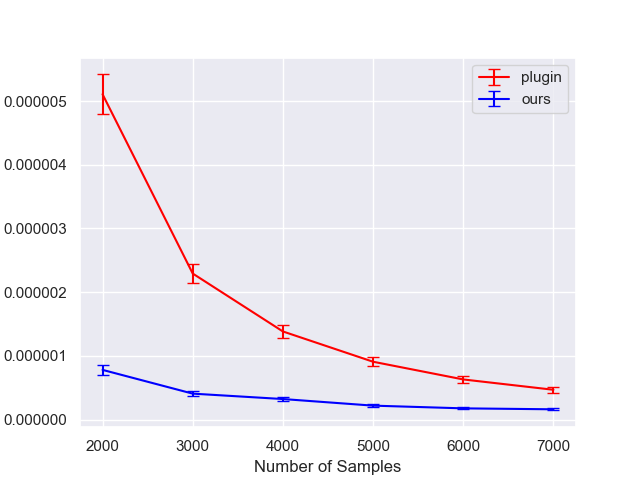
\includegraphics[width=\textwidth]{mse_estimator_100_bins.png}
         \caption{Mean-squared errors of estimates.}
         \label{fig:mse_estimators}
     \end{subfigure}
     \hfill
     \begin{subfigure}[b]{0.45\textwidth}
         \centering
         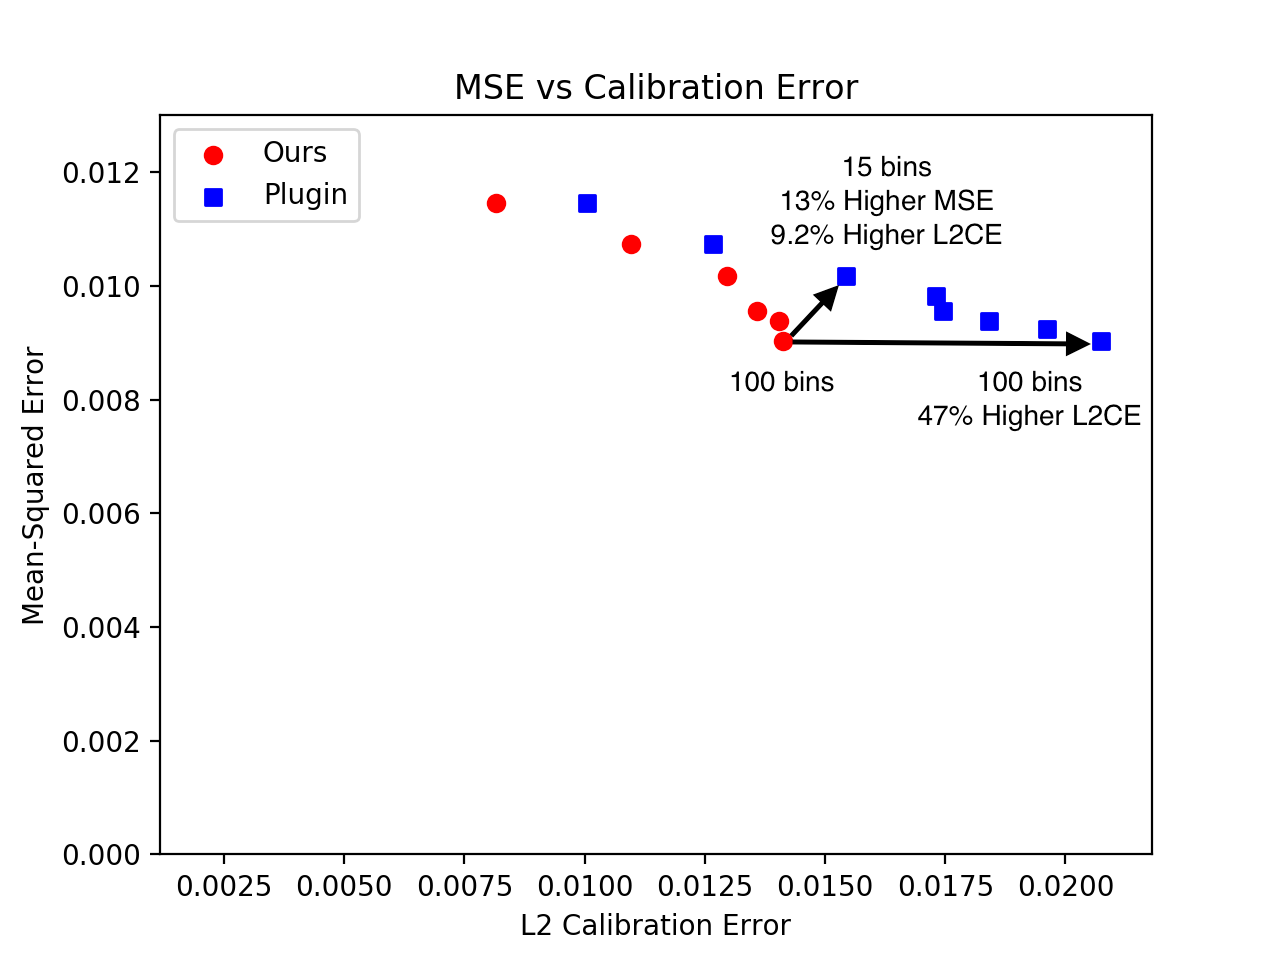
\includegraphics[width=\textwidth]{mse_vs_verified_error_plugin_vs_ours.png}
         \caption{Brier score vs calibration error.}
         \label{fig:mse_vs_ce_estimators}
     \end{subfigure}
  \caption{
  (\textbf{Left}) Mean-squared errors of cancelling and plugin estimators on a recalibrated VGG-net model on CIFAR-10 with $90\%$ confidence intervals (lower values better). Our estimator is closer to the ground truth.
  (\textbf{Right}) Plot of Brier scores against upper bounds on the calibration error computed by our estimator and the plugin estimator, when we vary the number of bins $B$. For a given calibration error, our estimator enables us to choose models with a better Brier score. If we want a model with $\ell_2$ calibration error less than 0.015, the cancelling estimator tells us we can confidently use 100 bins, while relying on the plugin estimator only lets us use 15 bins and incurs a 13\% higher Brier score.
  }
  \label{fig:mse_estimators_bins}
\end{figure}

% This means that our estimator has a substantially better dependency on the number of outputs of the model.

% \begin{corollary}
% \label{cor:final-ours}
% Using our estimator $\hat{E}$, if $n = \Theta(kb + \frac{\sqrt{b}}{\epsilon^2})$ ignoring $\log$ factors, we can check if $|{E^*} | \leq \epsilon$ with significance and power $\delta$, and constant effect size $r$. 
% \end{corollary}